\documentclass[aspectratio=169,11pt]{beamer}

% Theme and colors
\usetheme{Madrid}
\usecolortheme{whale}
\setbeamertemplate{navigation symbols}{}
\setbeamertemplate{footline}[frame number]

% Packages
\usepackage[utf8]{inputenc}
\usepackage[T1]{fontenc}
\usepackage{graphicx}
\usepackage{booktabs}
\usepackage{amsmath}
\usepackage{hyperref}
\usepackage{tikz}
\usetikzlibrary{shapes,arrows,positioning,calc,fit,backgrounds,decorations.pathreplacing,decorations.pathmorphing}
\usepackage{siunitx}

% Bibliography
\usepackage[backend=biber,style=ieee,sorting=none]{biblatex}
\addbibresource{references.bib}

% Custom colors for questions
\definecolor{questionbg}{RGB}{255,248,220}
\definecolor{questionborder}{RGB}{255,193,7}

% Title information
\title[EECE5155 -- Module 4]{Data Communication}
\subtitle{Module 4: From Local Processing to the Network}
\author{Eduardo Baena}
\date{Spring 2026}
\institute{Northeastern University\\Department of Electrical and Computer Engineering\\
\texttt{e.baena@northeastern.edu}}

\begin{document}

% Title slide
\begin{frame}
    \titlepage
    \vspace{-1cm}
    \begin{center}
        \textbf{EECE5155: Wireless Sensor Networks and the Internet of Things}
    \end{center}
\end{frame}

% Learning Objectives
\begin{frame}{Learning Objectives}
    \textbf{By the end of this module, you should be able to:}
    
    \vspace{0.5cm}
    \begin{enumerate}
        \item \textbf{Describe} the components of a wireless communication system
        \item \textbf{Calculate} energy consumption for transmission and reception
        \item \textbf{Compare} communication vs computation energy costs
        \item \textbf{Analyze} tradeoffs between sleep modes and startup energy
        \item \textbf{Apply} the energy model to your PES power budget
    \end{enumerate}
    
    \vspace{0.3cm}
    \begin{block}{Engineering Focus}
        Communication is often the \textbf{dominant energy consumer} in IoT. Your design decisions here determine battery life.
    \end{block}
\end{frame}

% Outline
\begin{frame}{Outline}
    \tableofcontents
\end{frame}

%==============================================================================
\section{Part 1: The Communications Unit}
%==============================================================================

\begin{frame}{Where Are We in the System?}
    \begin{center}
    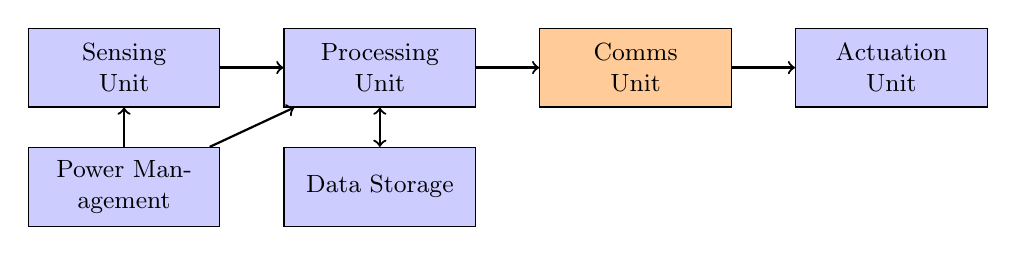
\begin{tikzpicture}[node distance=0.8cm, auto,
        block/.style={rectangle, draw, fill=blue!20, text width=2.2cm, text centered, minimum height=1cm, font=\small},
        highlight/.style={rectangle, draw, fill=orange!40, text width=2.2cm, text centered, minimum height=1cm, font=\small}]
        
        \node[block] (sense) {Sensing\\Unit};
        \node[block, right=of sense] (proc) {Processing\\Unit};
        \node[highlight, right=of proc] (comm) {Comms\\Unit};
        \node[block, right=of comm] (act) {Actuation\\Unit};
        \node[block, below=0.5cm of proc] (storage) {Data Storage};
        \node[block, below=0.5cm of sense] (power) {Power Management};
        
        \draw[->, thick] (sense) -- (proc);
        \draw[->, thick] (proc) -- (comm);
        \draw[->, thick] (comm) -- (act);
        \draw[<->, thick] (proc) -- (storage);
        \draw[->, thick] (power) -- (sense);
        \draw[->, thick] (power) -- (proc);
    \end{tikzpicture}
    \end{center}
    
    \vspace{0.3cm}
    \textbf{Today's focus:} The Communications Unit
    \begin{itemize}
        \item How do we get data from our ``Thing'' to the network?
        \item What are the energy implications?
    \end{itemize}
\end{frame}

%------------------------------------------------------------------------------
% QUESTION 1
%------------------------------------------------------------------------------
\begin{frame}{Think First}
    \begin{center}
    \fcolorbox{questionborder}{questionbg}{
    \begin{minipage}{0.85\textwidth}
        \vspace{0.3cm}
        \centering
        \Large\textbf{Question 1}
        
        \vspace{0.3cm}
        \normalsize
        In a battery-powered IoT sensor that samples temperature once per minute and transmits data:
        
        \vspace{0.3cm}
        \textbf{Which operation do you think consumes more energy?}
        
        \vspace{0.3cm}
        \begin{enumerate}[A)]
            \item Reading the temperature sensor
            \item Processing the data (averaging, formatting)
            \item Transmitting the data wirelessly
            \item Keeping the MCU in sleep mode
        \end{enumerate}
        \vspace{0.3cm}
    \end{minipage}
    }
    \end{center}
    
    \vspace{0.3cm}
    \textit{Discuss with your neighbor for 1 minute.}
\end{frame}

\begin{frame}{Answer: Communication Dominates}
    \textbf{C) Transmitting the data wirelessly}
    
    \vspace{0.3cm}
    \begin{table}
        \centering
        \begin{tabular}{@{}lccc@{}}
            \toprule
            \textbf{Operation} & \textbf{Power} & \textbf{Duration} & \textbf{Energy} \\
            \midrule
            Sensor read & 1 mA & 100 ms & 0.1 mJ \\
            Processing & 5 mA & 10 ms & 0.05 mJ \\
            \textbf{TX (LoRa)} & \textbf{120 mA} & \textbf{50 ms} & \textbf{6 mJ} \\
            Sleep (59.8 s) & 2 $\mu$A & 59.8 s & 0.12 mJ \\
            \bottomrule
        \end{tabular}
    \end{table}
    
    \vspace{0.3cm}
    \textbf{Key insight:} Radio transmission is typically \textbf{10--100$\times$} more expensive than local processing.
    
    \vspace{0.2cm}
    \begin{alertblock}{Engineering Implication}
        Minimize what you transmit. Process locally when possible.
    \end{alertblock}
\end{frame}

%------------------------------------------------------------------------------
% WHY COMMUNICATION
%------------------------------------------------------------------------------
\begin{frame}{Why Do We Need Communication?}
    \textbf{Not all IoT needs communication:}
    \begin{itemize}
        \item Smart thermostat: sense $\rightarrow$ process $\rightarrow$ actuate (local)
        \item Motion-activated light: sense $\rightarrow$ actuate (no processing needed)
    \end{itemize}
    
    \vspace{0.3cm}
    \textbf{But many applications require it:}
    \begin{itemize}
        \item \textbf{Multi-sensor coordination:} Data from multiple nodes needed
        \item \textbf{Remote monitoring:} Human needs to see data (dashboard)
        \item \textbf{Cloud analytics:} Complex ML requires more compute
        \item \textbf{Remote control:} Commands from user to device
        \item \textbf{Firmware updates:} Over-the-air updates
    \end{itemize}
    
    \vspace{0.3cm}
    \begin{block}{Your PES Question}
        Does your application \textit{require} communication? If yes, how much and how often?
    \end{block}
\end{frame}

%------------------------------------------------------------------------------
% PHYSICS OF WIRELESS
%------------------------------------------------------------------------------
\begin{frame}{Physics of Wireless Communication}
    \textbf{Different physical phenomena support wireless:}
    
    \vspace{0.3cm}
    \begin{table}
        \centering
        \small
        \begin{tabular}{@{}p{3cm}p{4cm}p{5cm}@{}}
            \toprule
            \textbf{Physics} & \textbf{Examples} & \textbf{IoT Use Case} \\
            \midrule
            Electromagnetic & Radio, microwave, mmWave & WiFi, BLE, LoRa, 5G \\
            \addlinespace
            Near-field magnetic & Magnetic induction & NFC, wireless charging \\
            \addlinespace
            Optical & Infrared, visible light & LiFi, IR remotes \\
            \addlinespace
            Acoustic & Sound, ultrasound & Underwater sensors \\
            \addlinespace
            Molecular & Ions, pheromones & Body area networks (research) \\
            \bottomrule
        \end{tabular}
    \end{table}
    
    \vspace{0.3cm}
    \textbf{This module:} Focus on electromagnetic (radio) -- dominant in IoT.
\end{frame}

%------------------------------------------------------------------------------
% TRANSCEIVER ARCHITECTURE
%------------------------------------------------------------------------------
\begin{frame}{Transceiver Architecture}
    \begin{center}
    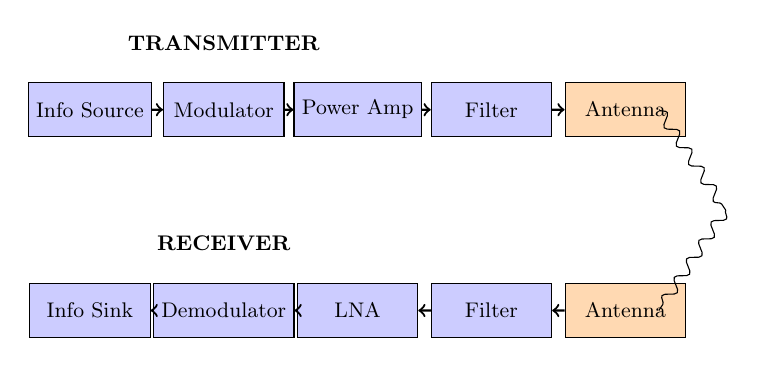
\begin{tikzpicture}[scale=0.85, transform shape,
        block/.style={rectangle, draw, fill=blue!20, minimum width=1.8cm, minimum height=0.8cm, font=\small},
        arrow/.style={->, thick}]
        
        % Transmitter
        \node[font=\small\bfseries] at (-4, 2.5) {TRANSMITTER};
        \node[block] (info1) at (-6, 1.5) {Info Source};
        \node[block] (mod) at (-4, 1.5) {Modulator};
        \node[block] (pa) at (-2, 1.5) {Power Amp};
        \node[block] (filt1) at (0, 1.5) {Filter};
        \node[block, fill=orange!30] (ant1) at (2, 1.5) {Antenna};
        
        \draw[arrow] (info1) -- (mod);
        \draw[arrow] (mod) -- (pa);
        \draw[arrow] (pa) -- (filt1);
        \draw[arrow] (filt1) -- (ant1);
        
        % Receiver
        \node[font=\small\bfseries] at (-4, -0.5) {RECEIVER};
        \node[block, fill=orange!30] (ant2) at (2, -1.5) {Antenna};
        \node[block] (filt2) at (0, -1.5) {Filter};
        \node[block] (lna) at (-2, -1.5) {LNA};
        \node[block] (demod) at (-4, -1.5) {Demodulator};
        \node[block] (info2) at (-6, -1.5) {Info Sink};
        
        \draw[arrow] (ant2) -- (filt2);
        \draw[arrow] (filt2) -- (lna);
        \draw[arrow] (lna) -- (demod);
        \draw[arrow] (demod) -- (info2);
        
        % RF waves
        \draw[decorate, decoration={snake, amplitude=2pt, segment length=8pt}] (2.5, 1.5) -- (3.5, 0);
        \draw[decorate, decoration={snake, amplitude=2pt, segment length=8pt}] (3.5, 0) -- (2.5, -1.5);
    \end{tikzpicture}
    \end{center}
    
    \vspace{0.2cm}
    \textbf{Key blocks:}
    \begin{itemize}
        \item \textbf{Modulator:} Encodes digital data onto carrier wave
        \item \textbf{Power Amplifier:} Boosts signal for transmission
        \item \textbf{LNA:} Low-Noise Amplifier -- amplifies weak received signal
        \item \textbf{Antenna:} Converts electrical signal $\leftrightarrow$ EM wave
    \end{itemize}
\end{frame}

%------------------------------------------------------------------------------
% QUESTION 2
%------------------------------------------------------------------------------
\begin{frame}{Think First}
    \begin{center}
    \fcolorbox{questionborder}{questionbg}{
    \begin{minipage}{0.85\textwidth}
        \vspace{0.3cm}
        \centering
        \Large\textbf{Question 2}
        
        \vspace{0.3cm}
        \normalsize
        A transceiver can be in these states: TX, RX, Idle, Sleep.
        
        \vspace{0.3cm}
        \textbf{Rank these states from highest to lowest power consumption:}
        
        \vspace{0.3cm}
        \begin{itemize}
            \item TX (transmitting)
            \item RX (receiving)
            \item Idle (ready to receive)
            \item Sleep (radio off)
        \end{itemize}
        \vspace{0.3cm}
    \end{minipage}
    }
    \end{center}
    
    \vspace{0.3cm}
    \textit{Write down your ranking before the next slide.}
\end{frame}

\begin{frame}{Answer: Transceiver States}
    \textbf{Typical ranking (highest to lowest power):}
    
    \vspace{0.3cm}
    \begin{table}
        \centering
        \begin{tabular}{@{}lcl@{}}
            \toprule
            \textbf{State} & \textbf{Typical Current} & \textbf{What's Active} \\
            \midrule
            TX & 20--150 mA & Everything + PA \\
            RX & 10--20 mA & LNA, demodulator, PLL \\
            Idle & 1--5 mA & Oscillator running, ready \\
            Sleep & 0.1--10 $\mu$A & Only wakeup circuit \\
            \bottomrule
        \end{tabular}
    \end{table}
    
    \vspace{0.3cm}
    \textbf{Surprise for many:} RX is often \textit{almost as expensive} as TX!
    
    \begin{itemize}
        \item TX power depends on output power (PA)
        \item At low TX power (0 dBm), TX $\approx$ RX
        \item At high TX power (+20 dBm), TX $>>$ RX
    \end{itemize}
    
    \vspace{0.2cm}
    \begin{alertblock}{Design Implication}
        Idle listening kills battery. Must use duty cycling or wake-up radios.
    \end{alertblock}
\end{frame}

%------------------------------------------------------------------------------
% TRANSCEIVER SPECS
%------------------------------------------------------------------------------
\begin{frame}{Transceiver Specifications for Your PES}
    \textbf{What you need to extract from datasheet:}
    
    \vspace{0.3cm}
    \begin{columns}[T]
        \begin{column}{0.48\textwidth}
            \textbf{RF Parameters:}
            \begin{itemize}
                \item Frequency band (MHz/GHz)
                \item Bandwidth (kHz/MHz)
                \item TX power (dBm)
                \item RX sensitivity (dBm)
                \item Modulation (FSK, LoRa, OFDM)
                \item Data rate (bps, kbps)
            \end{itemize}
        \end{column}
        \begin{column}{0.48\textwidth}
            \textbf{Power Parameters:}
            \begin{itemize}
                \item TX current at each power level
                \item RX current
                \item Idle current
                \item Sleep current
                \item Startup time (ms)
                \item Startup current
            \end{itemize}
        \end{column}
    \end{columns}
    
    \vspace{0.3cm}
    \begin{exampleblock}{Example: SX1276 (LoRa)}
        TX @ +14 dBm: 100 mA | RX: 10.8 mA | Sleep: 0.2 $\mu$A\\
        Sensitivity: -137 dBm (SF12) | Startup: 1.5 ms
    \end{exampleblock}
\end{frame}

%==============================================================================
\section{Energy Model for Communication}
%==============================================================================

%------------------------------------------------------------------------------
% UNITS REMINDER
%------------------------------------------------------------------------------
\begin{frame}{Quick Review: Power and Energy Units}
    \textbf{Make sure you're comfortable with these:}
    
    \vspace{0.3cm}
    \begin{columns}[T]
        \begin{column}{0.48\textwidth}
            \textbf{Linear units:}
            \begin{itemize}
                \item Power: Watts (W)
                \item Energy: Joules (J) = W $\cdot$ s
                \item Current: Amperes (A)
                \item $P = V \cdot I$
                \item $E = P \cdot t$
            \end{itemize}
        \end{column}
        \begin{column}{0.48\textwidth}
            \textbf{Logarithmic units:}
            \begin{itemize}
                \item dBm = $10 \log_{10}(P_{mW})$
                \item dBW = $10 \log_{10}(P_{W})$
                \item 0 dBm = 1 mW
                \item +20 dBm = 100 mW
                \item -10 dBm = 0.1 mW
            \end{itemize}
        \end{column}
    \end{columns}
    
    \vspace{0.3cm}
    \textbf{Conversions:}
    \begin{itemize}
        \item dBm to mW: $P_{mW} = 10^{dBm/10}$
        \item mW to dBm: $dBm = 10 \log_{10}(P_{mW})$
    \end{itemize}
\end{frame}

%------------------------------------------------------------------------------
% QUESTION 3
%------------------------------------------------------------------------------
\begin{frame}{Think First}
    \begin{center}
    \fcolorbox{questionborder}{questionbg}{
    \begin{minipage}{0.85\textwidth}
        \vspace{0.3cm}
        \centering
        \Large\textbf{Question 3}
        
        \vspace{0.3cm}
        \normalsize
        Your radio transmits at +14 dBm output power.\\
        The datasheet says TX current is 100 mA at 3.3V supply.
        
        \vspace{0.3cm}
        \textbf{What is the efficiency of the power amplifier?}
        
        \vspace{0.2cm}
        Hint: Efficiency = $\frac{P_{out}}{P_{in}} \times 100\%$
        
        \vspace{0.3cm}
        \begin{enumerate}[A)]
            \item $\approx$ 1\%
            \item $\approx$ 8\%
            \item $\approx$ 25\%
            \item $\approx$ 75\%
        \end{enumerate}
        \vspace{0.3cm}
    \end{minipage}
    }
    \end{center}
\end{frame}

\begin{frame}{Answer: PA Efficiency}
    \textbf{B) $\approx$ 8\%}
    
    \vspace{0.3cm}
    \textbf{Calculation:}
    \begin{align*}
        P_{out} &= 10^{14/10} \text{ mW} = 25 \text{ mW} \\
        P_{in} &= V \cdot I = 3.3 \text{ V} \times 100 \text{ mA} = 330 \text{ mW} \\
        \eta &= \frac{25}{330} \times 100\% = 7.6\%
    \end{align*}
    
    \vspace{0.3cm}
    \textbf{Where does the other 92\% go?}
    \begin{itemize}
        \item PA inefficiency (heat)
        \item Oscillators, PLLs, synthesizers
        \item Digital baseband processing
        \item Voltage regulators
    \end{itemize}
    
    \vspace{0.2cm}
    \begin{alertblock}{Engineering Reality}
        Most energy is \textit{not} radiated -- it's consumed by the radio electronics.
    \end{alertblock}
\end{frame}

%------------------------------------------------------------------------------
% ENERGY MODEL
%------------------------------------------------------------------------------
\begin{frame}{Energy Model for Communication}
    \textbf{Total communication energy:}
    
    \vspace{0.3cm}
    \[
    E_c = N_T \left[ P_{te}(T_{on} + T_{st}) + P_O \cdot T_{on} \right] + N_R \left[ P_{re}(R_{on} + R_{st}) \right]
    \]
    
    \vspace{0.3cm}
    \begin{columns}[T]
        \begin{column}{0.48\textwidth}
            \textbf{Transmitter:}
            \begin{itemize}
                \item $P_{te}$: TX electronics power
                \item $P_O$: Output power
                \item $T_{on}$: TX ``on'' time
                \item $T_{st}$: TX startup time
                \item $N_T$: Number of TX events
            \end{itemize}
        \end{column}
        \begin{column}{0.48\textwidth}
            \textbf{Receiver:}
            \begin{itemize}
                \item $P_{re}$: RX electronics power
                \item $R_{on}$: RX ``on'' time
                \item $R_{st}$: RX startup time
                \item $N_R$: Number of RX events
            \end{itemize}
        \end{column}
    \end{columns}
    
    \vspace{0.3cm}
    \textbf{Key insight:} $T_{on} = L / R$ where $L$ = packet size (bits), $R$ = data rate (bps)
\end{frame}

%------------------------------------------------------------------------------
% QUESTION 4
%------------------------------------------------------------------------------
\begin{frame}{Think First}
    \begin{center}
    \fcolorbox{questionborder}{questionbg}{
    \begin{minipage}{0.85\textwidth}
        \vspace{0.3cm}
        \centering
        \Large\textbf{Question 4}
        
        \vspace{0.3cm}
        \normalsize
        You need to transmit 100 bytes of sensor data.\\
        Your radio has:
        \begin{itemize}
            \item Startup time: 1 ms at 30 mA
            \item TX current: 100 mA
            \item Data rate: 10 kbps
        \end{itemize}
        
        \vspace{0.3cm}
        \textbf{What percentage of TX energy is ``wasted'' on startup?}
        
        \vspace{0.3cm}
        \begin{enumerate}[A)]
            \item $\approx$ 0.4\%
            \item $\approx$ 4\%
            \item $\approx$ 27\%
            \item $\approx$ 50\%
        \end{enumerate}
        \vspace{0.3cm}
    \end{minipage}
    }
    \end{center}
\end{frame}

\begin{frame}{Answer: Startup Energy Overhead}
    \textbf{A) $\approx$ 0.4\% -- for this packet size}
    
    \vspace{0.3cm}
    \textbf{Calculation:}
    \begin{align*}
        T_{on} &= \frac{100 \times 8 \text{ bits}}{10000 \text{ bps}} = 80 \text{ ms} \\
        E_{startup} &= 30 \text{ mA} \times 1 \text{ ms} = 0.03 \text{ mA} \cdot \text{s} \\
        E_{TX} &= 100 \text{ mA} \times 80 \text{ ms} = 8 \text{ mA} \cdot \text{s} \\
        \text{Startup \%} &= \frac{0.03}{8.03} \times 100\% = 0.37\%
    \end{align*}
    
    \vspace{0.3cm}
    \textbf{But what if packet is only 10 bytes?}
    \begin{itemize}
        \item $T_{on}$ = 8 ms, $E_{TX}$ = 0.8 mA$\cdot$s
        \item Startup \% = 3.6\%
    \end{itemize}
    
    \begin{alertblock}{Key Insight}
        Startup overhead becomes significant for small packets. Batch data when possible!
    \end{alertblock}
\end{frame}

\begin{frame}{Startup Energy vs Packet Size}
    \begin{center}
    \begin{tikzpicture}[scale=0.9]
        \draw[->] (0,0) -- (10,0) node[right] {Packet Size (bits)};
        \draw[->] (0,0) -- (0,5) node[above] {Energy/bit};
        
        % Curve showing decreasing energy per bit
        \draw[thick, blue] plot[smooth] coordinates {(0.5,4.5) (1,3) (2,2) (3,1.5) (4,1.2) (5,1) (6,0.9) (7,0.85) (8,0.82) (9,0.8)};
        
        % Asymptote
        \draw[dashed, red] (0,0.8) -- (10,0.8) node[right] {$E_{elec}$};
        
        % Annotations
        \node[align=center, font=\small] at (2,3.5) {Startup\\dominates};
        \node[align=center, font=\small] at (7,1.8) {TX time\\dominates};
        
        % X-axis labels
        \node[below, font=\tiny] at (1,0) {10};
        \node[below, font=\tiny] at (3,0) {100};
        \node[below, font=\tiny] at (5,0) {1000};
        \node[below, font=\tiny] at (7,0) {10000};
    \end{tikzpicture}
    \end{center}
    
    \vspace{0.2cm}
    \textbf{As packet size decreases:}
    \begin{itemize}
        \item Fixed startup cost is amortized over fewer bits
        \item Energy per bit increases dramatically
        \item Inefficient to send many small packets
    \end{itemize}
    
    \textbf{Design implication:} Buffer data and send larger, less frequent packets.
\end{frame}

%------------------------------------------------------------------------------
% SLEEP VS STARTUP TRADEOFF
%------------------------------------------------------------------------------
\begin{frame}{The Sleep vs Startup Tradeoff}
    \begin{center}
    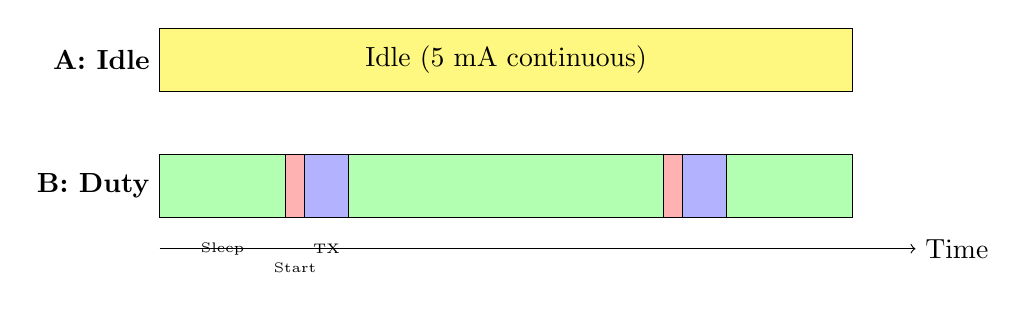
\begin{tikzpicture}[scale=0.8]
        % Timeline
        \draw[->] (0,0) -- (12,0) node[right] {Time};
        
        % Option A: Always on
        \node[left] at (0,3) {\textbf{A: Idle}};
        \draw[fill=yellow!50] (0,2.5) rectangle (11,3.5);
        \node at (5.5,3) {Idle (5 mA continuous)};
        
        % Option B: Sleep/Wake
        \node[left] at (0,1) {\textbf{B: Duty}};
        \draw[fill=green!30] (0,0.5) rectangle (2,1.5);
        \draw[fill=red!30] (2,0.5) rectangle (2.3,1.5);
        \draw[fill=blue!30] (2.3,0.5) rectangle (3,1.5);
        \draw[fill=green!30] (3,0.5) rectangle (8,1.5);
        \draw[fill=red!30] (8,0.5) rectangle (8.3,1.5);
        \draw[fill=blue!30] (8.3,0.5) rectangle (9,1.5);
        \draw[fill=green!30] (9,0.5) rectangle (11,1.5);
        
        % Legend
        \node[font=\tiny] at (1,0) {Sleep};
        \node[font=\tiny] at (2.15,-0.3) {Start};
        \node[font=\tiny] at (2.65,0) {TX};
    \end{tikzpicture}
    \end{center}
    
    \vspace{0.2cm}
    \textbf{When is duty cycling worth it?}
    
    When: $E_{sleep} + E_{startup} < E_{idle}$ over the same period
    
    \vspace{0.3cm}
    \textbf{Break-even calculation:}
    \begin{itemize}
        \item If idle = 5 mA, sleep = 1 $\mu$A, startup = 2 mA for 1 ms
        \item Savings per second of sleep: 5 mA - 0.001 mA = 4.999 mA
        \item Startup cost: 2 mA $\times$ 1 ms = 0.002 mA$\cdot$s
        \item Break-even: 0.002/4.999 = 0.4 ms $\rightarrow$ Always worth it if sleep > 0.4 ms!
    \end{itemize}
\end{frame}

%==============================================================================
\section{Communication vs Computation Energy}
%==============================================================================

%------------------------------------------------------------------------------
% QUESTION 5
%------------------------------------------------------------------------------
\begin{frame}{Think First}
    \begin{center}
    \fcolorbox{questionborder}{questionbg}{
    \begin{minipage}{0.85\textwidth}
        \vspace{0.3cm}
        \centering
        \Large\textbf{Question 5}
        
        \vspace{0.3cm}
        \normalsize
        You have a sensor node that generates 1 KB of data.\\
        You can either:
        \begin{itemize}
            \item[A)] Send all 1 KB to the cloud
            \item[B)] Process locally to extract 10-byte summary, send summary
        \end{itemize}
        
        \vspace{0.3cm}
        Local processing takes 10 ms at 5 mA.\\
        Radio TX takes 100 mA and sends at 10 kbps.
        
        \vspace{0.3cm}
        \textbf{Which option uses less energy?}
        \vspace{0.3cm}
    \end{minipage}
    }
    \end{center}
\end{frame}

\begin{frame}{Answer: Local Processing Wins}
    \textbf{Option B uses $\sim$16$\times$ less energy!}
    
    \vspace{0.3cm}
    \textbf{Option A: Send all data}
    \begin{align*}
        T_{TX} &= \frac{1024 \times 8}{10000} = 819 \text{ ms} \\
        E_A &= 100 \text{ mA} \times 819 \text{ ms} = 81.9 \text{ mA} \cdot \text{ms}
    \end{align*}
    
    \textbf{Option B: Process + send summary}
    \begin{align*}
        E_{proc} &= 5 \text{ mA} \times 10 \text{ ms} = 0.05 \text{ mA} \cdot \text{ms} \\
        T_{TX} &= \frac{10 \times 8}{10000} = 8 \text{ ms} \\
        E_{TX} &= 100 \text{ mA} \times 8 \text{ ms} = 0.8 \text{ mA} \cdot \text{ms} \\
        E_B &= 0.05 + 0.8 = 0.85 \text{ mA} \cdot \text{ms}
    \end{align*}
    
    \begin{block}{Edge Computing Principle}
        \textbf{Compute is cheap, communication is expensive.} Always minimize TX data.
    \end{block}
\end{frame}

\begin{frame}{The Famous Comparison}
    \textbf{Classic result from WSN literature:}
    
    \vspace{0.3cm}
    \begin{quote}
        ``The energy cost of transmitting 1 KB over 100 meters is approximately equal to executing \textbf{3 million instructions} on a 100 MIPS processor.''
    \end{quote}
    
    \vspace{0.3cm}
    \textbf{Assumptions:}
    \begin{itemize}
        \item Traditional radio at 1--2 GHz
        \item Rayleigh fading channel, path loss $\propto d^4$
        \item Low-power MCU
    \end{itemize}
    
    \vspace{0.3cm}
    \begin{alertblock}{Implication for Your PES}
        Can you reduce TX data by 10$\times$ with local processing?\\
        If yes, you extend battery life significantly -- \textbf{document this tradeoff!}
    \end{alertblock}
\end{frame}

%------------------------------------------------------------------------------
% COMPUTATION ENERGY MODEL
%------------------------------------------------------------------------------
\begin{frame}{Energy Model for Computation}
    \textbf{Processing energy:}
    
    \[
    E_p = N \cdot C \cdot V_{dd}^2 + V_{dd} \cdot I_O \cdot e^{\frac{V_{dd}}{n \cdot V_T}} \cdot \frac{1}{f}
    \]
    
    \vspace{0.2cm}
    \begin{columns}[T]
        \begin{column}{0.48\textwidth}
            \textbf{Dynamic power} (first term):
            \begin{itemize}
                \item $N$: Clock cycles per task
                \item $C$: Capacitance per cycle
                \item $V_{dd}$: Supply voltage
            \end{itemize}
        \end{column}
        \begin{column}{0.48\textwidth}
            \textbf{Leakage} (second term):
            \begin{itemize}
                \item $I_O$: Leakage current
                \item $V_T$: Thermal voltage
                \item $n$: Ideality factor
                \item $\approx$10\% of total
            \end{itemize}
        \end{column}
    \end{columns}
    
    \vspace{0.3cm}
    \textbf{Practical implication:} $E \propto V^2$
    
    Lower voltage = quadratically lower energy (but slower)
\end{frame}

\begin{frame}{Real MCU Power Numbers}
    \begin{table}
        \centering
        \begin{tabular}{@{}lccc@{}}
            \toprule
            \textbf{MCU} & \textbf{Active} & \textbf{Sleep} & \textbf{Deep Sleep} \\
            \midrule
            TI MSP430 (1 MHz, 3V) & 1.2 mW & -- & 0.3 $\mu$W \\
            Atmel ATmega328 & 15 mW & 6 mW & 75 $\mu$W \\
            STM32L072 (32 MHz) & 10 mW & 1.2 $\mu$W & 0.3 $\mu$W \\
            ESP32 (240 MHz) & 260 mW & 5 $\mu$W & 2.5 $\mu$W \\
            nRF52840 (64 MHz) & 16.5 mW & 1.5 $\mu$W & 0.4 $\mu$W \\
            \bottomrule
        \end{tabular}
    \end{table}
    
    \vspace{0.3cm}
    \textbf{Observations:}
    \begin{itemize}
        \item Active power varies 20$\times$ across MCUs
        \item Sleep modes vary 1000$\times$ -- \textbf{this matters for IoT!}
        \item Deep sleep: only wakeup timer/interrupt active
    \end{itemize}
\end{frame}

%------------------------------------------------------------------------------
% DVS
%------------------------------------------------------------------------------
\begin{frame}{Dynamic Voltage Scaling (DVS)}
    \textbf{Trade speed for power:}
    
    \vspace{0.3cm}
    \begin{center}
    \begin{tikzpicture}[scale=0.8]
        \draw[->] (0,0) -- (6,0) node[right] {Frequency};
        \draw[->] (0,0) -- (0,4) node[above] {Power};
        
        % Power curve (cubic relationship)
        \draw[thick, blue] plot[smooth, domain=0.5:5] (\x, {0.1*\x*\x*\x});
        
        % Points
        \fill[red] (4,6.4/4) circle (3pt) node[above right] {High f, high P};
        \fill[green] (2,0.8/4) circle (3pt) node[above right] {Low f, low P};
        
        \node[align=left, font=\small] at (8,3) {$P \propto f \cdot V^2$\\$V_{min} \propto f$\\$\therefore P \propto f^3$};
    \end{tikzpicture}
    \end{center}
    
    \vspace{0.2cm}
    \textbf{Example:}
    \begin{itemize}
        \item Run at 100 MHz, 1.2V: $P_1 = 10$ mW, task takes 10 ms $\rightarrow E = 100 \mu$J
        \item Run at 50 MHz, 0.9V: $P_2 = 2.8$ mW, task takes 20 ms $\rightarrow E = 56 \mu$J
    \end{itemize}
    
    \textbf{Lower frequency = lower energy!} (if you have time)
\end{frame}

%==============================================================================
\section{Memory and Total Energy Model}
%==============================================================================

\begin{frame}{Memory Energy: Flash vs RAM}
    \begin{table}
        \centering
        \begin{tabular}{@{}lcc@{}}
            \toprule
            \textbf{Operation} & \textbf{Energy} & \textbf{Notes} \\
            \midrule
            RAM read/write & $\approx$ 1 nJ/byte & Negligible \\
            Flash read & 1.1 nAh/byte & $\approx$ 4 nJ/byte @ 3.3V \\
            Flash write/erase & 83.3 nAh/byte & $\approx$ 300 nJ/byte @ 3.3V \\
            \bottomrule
        \end{tabular}
    \end{table}
    
    \vspace{0.3cm}
    \textbf{Flash write is 75$\times$ more expensive than read!}
    
    \vspace{0.3cm}
    \textbf{Design implications:}
    \begin{itemize}
        \item Buffer data in RAM, batch write to Flash
        \item Avoid excessive logging to Flash
        \item Use wear leveling for long-term storage
    \end{itemize}
    
    \vspace{0.2cm}
    \begin{block}{For Your PES}
        If logging data: calculate Flash write energy. It can be significant!
    \end{block}
\end{frame}

%------------------------------------------------------------------------------
% QUESTION 6
%------------------------------------------------------------------------------
\begin{frame}{Think First}
    \begin{center}
    \fcolorbox{questionborder}{questionbg}{
    \begin{minipage}{0.85\textwidth}
        \vspace{0.3cm}
        \centering
        \Large\textbf{Question 6: Complete Energy Budget}
        
        \vspace{0.3cm}
        \normalsize
        A sensor node does this once per minute:
        \begin{itemize}
            \item Read sensor: 1 mA for 100 ms
            \item Process data: 5 mA for 10 ms
            \item Transmit 50 bytes: 100 mA for 40 ms
            \item Sleep: 2 $\mu$A for 59.85 s
        \end{itemize}
        
        \vspace{0.3cm}
        Battery: 1000 mAh
        
        \vspace{0.3cm}
        \textbf{How long will the battery last?}
        \vspace{0.3cm}
    \end{minipage}
    }
    \end{center}
\end{frame}

\begin{frame}{Answer: Battery Life Calculation}
    \textbf{Step 1: Energy per cycle}
    \begin{align*}
        E_{sense} &= 1 \text{ mA} \times 100 \text{ ms} = 0.1 \text{ mA} \cdot \text{ms} \\
        E_{proc} &= 5 \text{ mA} \times 10 \text{ ms} = 0.05 \text{ mA} \cdot \text{ms} \\
        E_{TX} &= 100 \text{ mA} \times 40 \text{ ms} = 4.0 \text{ mA} \cdot \text{ms} \\
        E_{sleep} &= 0.002 \text{ mA} \times 59850 \text{ ms} = 0.12 \text{ mA} \cdot \text{ms} \\
        E_{total} &= 4.27 \text{ mA} \cdot \text{ms per minute}
    \end{align*}
    
    \textbf{Step 2: Average current}
    \[
    I_{avg} = \frac{4.27 \text{ mA} \cdot \text{ms}}{60000 \text{ ms}} = 71.2 \text{ } \mu\text{A}
    \]
    
    \textbf{Step 3: Battery life}
    \[
    t = \frac{1000 \text{ mAh}}{0.0712 \text{ mA}} = 14,045 \text{ h} = \textbf{1.6 years}
    \]
\end{frame}

%==============================================================================
\section{Simple Energy Model}
%==============================================================================

\begin{frame}{A Simple First-Order Model}
    \textbf{For quick calculations:}
    
    \vspace{0.3cm}
    \begin{columns}[T]
        \begin{column}{0.48\textwidth}
            \textbf{Transmit energy:}
            \[
            E_{TX}(k,d) = E_{elec} \cdot k + E_{amp} \cdot k \cdot d^2
            \]
            
            \textbf{Receive energy:}
            \[
            E_{RX}(k) = E_{elec} \cdot k
            \]
        \end{column}
        \begin{column}{0.48\textwidth}
            \textbf{Typical values:}
            \begin{itemize}
                \item $E_{elec}$ = 50 nJ/bit
                \item $E_{amp}$ = 100 pJ/bit/m$^2$
                \item $k$ = packet size (bits)
                \item $d$ = distance (m)
            \end{itemize}
        \end{column}
    \end{columns}
    
    \vspace{0.3cm}
    \begin{center}
    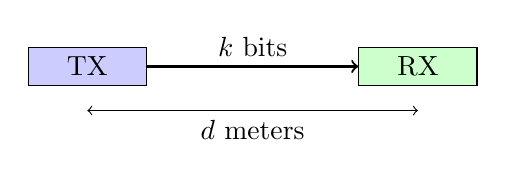
\begin{tikzpicture}[scale=0.7]
        \node[draw, rectangle, fill=blue!20, minimum width=1.5cm] (tx) at (0,0) {TX};
        \node[draw, rectangle, fill=green!20, minimum width=1.5cm] (rx) at (6,0) {RX};
        \draw[->, thick] (tx) -- (rx) node[midway, above] {$k$ bits};
        \draw[<->] (0,-0.8) -- (6,-0.8) node[midway, below] {$d$ meters};
    \end{tikzpicture}
    \end{center}
\end{frame}

%------------------------------------------------------------------------------
% QUESTION 7
%------------------------------------------------------------------------------
\begin{frame}{Think First}
    \begin{center}
    \fcolorbox{questionborder}{questionbg}{
    \begin{minipage}{0.85\textwidth}
        \vspace{0.3cm}
        \centering
        \Large\textbf{Question 7}
        
        \vspace{0.3cm}
        \normalsize
        Using the simple model ($E_{elec}$ = 50 nJ/bit, $E_{amp}$ = 100 pJ/bit/m$^2$):
        
        \vspace{0.3cm}
        Transfer 1 Mbit from source to sink, 100 m apart.\\
        Each node has 5 m broadcast radius.\\
        Neighbors can overhear broadcasts.
        
        \vspace{0.3cm}
        \begin{center}
        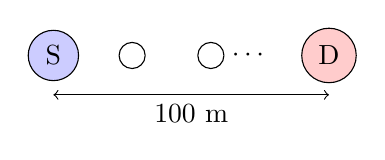
\begin{tikzpicture}[scale=0.5]
            \node[draw, circle, fill=blue!20] (s) at (0,0) {S};
            \node[draw, circle] (n1) at (2,0) {};
            \node[draw, circle] (n2) at (4,0) {};
            \node at (5,0) {$\cdots$};
            \node[draw, circle, fill=red!20] (d) at (7,0) {D};
            \draw[<->] (0,-1) -- (7,-1) node[midway, below] {100 m};
        \end{tikzpicture}
        \end{center}
        
        \textbf{What is the total energy to deliver the data?}
        \vspace{0.3cm}
    \end{minipage}
    }
    \end{center}
\end{frame}

\begin{frame}{Answer: Multi-hop Energy}
    \textbf{Setup:}
    \begin{itemize}
        \item Distance: 100 m, hop distance: 5 m
        \item Number of hops: 100/5 = 20 hops
        \item Each hop: 1 TX + multiple RX (neighbors overhear)
    \end{itemize}
    
    \vspace{0.3cm}
    \textbf{Energy per hop:}
    \begin{align*}
        E_{TX} &= 50 \text{ nJ/bit} \times 10^6 + 100 \text{ pJ/bit/m}^2 \times 10^6 \times 5^2 \\
               &= 50 \text{ mJ} + 2.5 \text{ mJ} = 52.5 \text{ mJ}
    \end{align*}
    
    \textbf{Total for 20 hops (TX only):}
    \[
    E_{total,TX} = 20 \times 52.5 \text{ mJ} = 1.05 \text{ J}
    \]
    
    \textbf{Plus RX energy} (assume 2 neighbors per hop overhear):
    \[
    E_{total,RX} = 20 \times 3 \times 50 \text{ mJ} = 3 \text{ J}
    \]
    
    \textbf{Total: $\approx$ 4 J} (RX dominates due to overhearing!)
\end{frame}

%==============================================================================
\section{Summary and PES Integration}
%==============================================================================

\begin{frame}{Key Takeaways for Your PES}
    \begin{enumerate}
        \item \textbf{Communication dominates energy budget}
        \begin{itemize}
            \item TX and RX are 10--100$\times$ more expensive than processing
        \end{itemize}
        
        \item \textbf{Sleep current matters most for duty-cycled systems}
        \begin{itemize}
            \item Compare sleep currents when selecting radios
        \end{itemize}
        
        \item \textbf{Startup overhead matters for small packets}
        \begin{itemize}
            \item Batch data when possible
        \end{itemize}
        
        \item \textbf{Local processing saves energy}
        \begin{itemize}
            \item Compute is cheap, bandwidth is expensive
        \end{itemize}
        
        \item \textbf{Document your energy budget with sources}
        \begin{itemize}
            \item Every current value needs a datasheet reference
        \end{itemize}
    \end{enumerate}
\end{frame}

\begin{frame}{What Your PES Section 7 Must Include}
    \textbf{Communication System:}
    
    \vspace{0.3cm}
    \begin{enumerate}
        \item \textbf{Radio selected:} Part number, why this one?
        
        \item \textbf{Power analysis:} (from datasheet)
        \begin{itemize}
            \item TX current at chosen power level
            \item RX current
            \item Sleep current
            \item Startup time and current
        \end{itemize}
        
        \item \textbf{Protocol parameters:}
        \begin{itemize}
            \item Packet size, data rate
            \item TX/RX events per hour/day
        \end{itemize}
        
        \item \textbf{Energy calculation:}
        \begin{itemize}
            \item Energy per TX/RX event
            \item Average current contribution
            \item Impact on battery life
        \end{itemize}
    \end{enumerate}
\end{frame}

\begin{frame}{What's Next}
    \textbf{Module 4 - Part 2: Protocols and Standards}
    
    \vspace{0.3cm}
    \begin{itemize}
        \item WiFi, BLE, Zigbee, LoRa, NB-IoT, LTE-M
        \item Protocol selection criteria
        \item Link budgets and range calculations
        \item Network topologies
    \end{itemize}
    
    \vspace{0.5cm}
    \begin{center}
        \Large
        \textbf{Questions?}
    \end{center}
\end{frame}

%==============================================================================
% References
%==============================================================================

\begin{frame}[allowframebreaks]{References}
    \printbibliography
\end{frame}

\end{document}
